documentclass{article}
\usepackage{pdfsync}
\usepackage{enumerate}
\usepackage{listings}  % Include the listings-package
\usepackage{framed}
\usepackage{float}
\usepackage{amsmath}
\usepackage{dsfont}
\usepackage{bm}
\usepackage{multicol}
\usepackage{subcaption}
\usepackage{enumitem}
\usepackage[compact]{titlesec}
\usepackage{wrapfig}
\usepackage{mdframed}
\usepackage{placeins}

\newenvironment{bprob}
    {\begin{mdframed}
    }
    {
   \end{mdframed}
    }

\lstset{
    language=Python,
    numbers=left,
    stepnumber=1,
    showstringspaces=false,
    tabsize=4,
    breaklines=true,
    breakatwhitespace=false,
    columns=fullflexible,
    basicstyle=\footnotesize\ttfamily
}

\usepackage{amsmath,amsfonts,amsthm,amssymb,amsopn,bm}
\usepackage[margin=.9in]{geometry}
\usepackage{graphicx}
\usepackage{url}
\newtheorem{lemma}{Lemma}
\usepackage{fancyhdr}
\usepackage[ruled]{algorithm2e}
\usepackage{multirow}
\newcommand{\field}[1]{\mathbb{#1}}
\newcommand{\1}{\mathbf{1}}
\renewcommand{\P}{\mathbb{P}}
\newcommand{\F}{\field{F}}
\newcommand{\T}{^{\textrm T}} % transpose

\def\diag{\text{diag}}

%% operator in linear algebra, functional analysis
\newcommand{\inner}[2]{#1\cdot #2}
\newcommand{\norm}[1]{\left\|#1\right\|}
\newcommand{\twonorm}[1]{\|#1\|_2^2}
% operator in functios, maps such as M: domain1 --> domain 2
\newcommand{\Map}[1]{\mathcal{#1}}
\renewcommand{\theenumi}{\alph{enumi}} 

\newcommand{\Perp}{\perp \! \! \! \perp}

\def\E{\mathbb{E}}
\def\P{\mathbb{P}}
\def\R{\mathbb{R}}
\newcommand{\mb}[1]{\mathbf{#1}}
\newcommand{\mc}[1]{\mathcal{#1}}

\newcommand\independent{\protect\mathpalette{\protect\independenT}{\perp}}
\def\independenT#1#2{\mathrel{\rlap{$#1#2$}\mkern2mu{#1#2}}}
\newcommand{\vct}[1]{\boldsymbol{#1}} % vector
\newcommand{\mat}[1]{\boldsymbol{#1}} % matrix
\newcommand{\cst}[1]{\mathsf{#1}} % constant
\newcommand{\ProbOpr}[1]{\mathbb{#1}}
\def\r{\textcolor{red}}
\newcommand{\points}[1]{\small\textcolor{magenta}{\emph{[#1 points]}} \normalsize}
\date{{}}
\setlength\parindent{0px}


\begin{document}
\title{Homework \#3} 
\author{\normalsize{CSE 446: Machine Learning}\\ 
\normalsize{Eric Boris: 1976637}}
%\normalsize{Collaborators:}
\maketitle

% \noindent Please review all homework guidance posted on the website before
submitting to Gradescope.  Reminders:
\begin{itemize}
  \item Please provide succinct answers along with
succinct reasoning for all your answers. Points may be deducted if
long answers demonstrate a lack of clarity. Similarly, when discussing
the experimental results, concisely create tables and/or figures when
appropriate to organize the experimental results. In other words, all
your explanations, tables, and figures for any particular part of a
question must be grouped together.
\item For every problem involving generating plots, please include the plots as part of your PDF subm
\item When submitting to gradescope, please link each question from the homework in gradescope to the
\item Please include all your code for programming problems. We may run your code to check the correc
\item All work must be typeset. We recommend using \LaTeX, but Google Docs, Microsoft Word, etc, are
\item All code questions must be typed in Python. We don't accept any other languages.
\item If you collaborate on this homework with others, you must indicate who you worked with on your
\end{itemize}


\section*{Conceptual Questions}
\noindent\rule{\textwidth}{1pt}\vspace{0.75mm}
{\bf Problem 0}
\begin{enumerate}
    \item {\bf No}, because it's possible that there are other highly correlated features that also have large positive weights. In which case, any one could be removed without affecting the quality of the predictions. 

    \item The L1 norm penalty results in a more sparse features than the L2 norm because the {\bf L1 ball is diamond shaped with vertices on the axes} while the {\bf L2 norm is spherical}. This means that an intersection between the function's contour lines with the L1 ball are more likely to occur on an axis, resulting in zeros for the other axes, than with the L2 norm.


    \item Advantage: Better {\bf weight sparsity} than L1. Disadvantage: {\bf Non-Convex}.

    \item k-fold cross validation works by dividing the training data into k subsets. 
For k iterations, one of the k subsets is used as a test set and the model is trained over the remaining k-1 subsets. 
The resulting error is found by averaging the error over the k iterations. 
{\bf Because the training set using k-fold cross is smaller}, k-1 than for example n-1 as in LOOCV, {\bf the bias is higher}. 
But training time is reduced for k-fold cross from LOOCV.
In short, increasing k increases the size of the training set and therefore, increases training time and reduces bias. 
{\bf k=10} could be a reasonable choice because k is sufficiently large to have {\bf low bias but fast training times}.



    \item {\bf True} because the gradient update values can get stuck stepping over the minimum.

    \item Because {\bf on average it goes in the direction of the true gradient}.

    \item Advantage: SGD is {\bf less computationally intensive} than GD. Disadvantage: SGD requires {\bf more training} than GD to achieve the same error.

\end{enumerate}


\section*{Convexity and Norms}
\noindent\rule{\textwidth}{1pt}\vspace{0.75mm}
\section{}
We are given the probability of having a certain disease $P(x) = 0.0001$. From this we know the probability of not having the disease $P(\overline{x}) = 0.9999$. We are given the probability of testing positive given that we have the disease $P(y | x) = 0.99$ and we are given the probability of testing negative given that we don't have the disease $P(\overline{y} | \overline{x}) = 0.99$. From these we know the probability of testing positive given that we don't have the disease $P(y | \overline{x}) = 0.01$ and the probability of testing negative given that have the disease $P(\overline{y} | x) = 0.01$. We use Bayes' Rule to determine our probability of having the disease given that we test positive $P(x | y)$.

\begin{align*}
    P(x | y)
	&= \frac{P(x, y)}{P(y)} \tag*{Bayes' Rule} \\
	&= \frac{P(x)P(y|x)}{P(\overline{x})P(y | \overline{x}) + P(x)P(y|x)} \\
	&= \frac{(0.0001)(0.99)}{(0.9999)(0.01) + (0.0001)(0.99)} \tag*{Substitution} \\
	&= \frac{1}{102} \\
	&\approx 0.0098
\end{align*}


\noindent\rule{\textwidth}{1pt}\vspace{0.75mm}
2. Consider a model consisting of random variables $X, Y$ and $Z$: $Y = Xw + Z$, where $Z \sim U[-0.5, 0.5]$. Assume that $Z$ is a noise here (i.e. the independence holds) and $w \in \mathbb{R}$ is a fixed parameter (i.e. it is not random).

\begin{enumerate}
    \item \points{5} Derive the probability density function (pdf) of $Y$ conditioning on $\{X = x\}$.
	\begin{itemize}
    \item[] Given that $Z \sim U[-0.5, 0.5]$, we write the PDF as:
	\begin{equation*}
	    P(Z = z) = 
	    \left\{
		\begin{array}{ll}
		    1 & \lvert z \rvert \leq 0.5 \\
		    0 & \textrm{otherwise}
		\end{array}
	    \right.
	\end{equation*}
    \item[] Given that $Y = Xw + Z \implies Z = Y - Xw$, we write the PDF as:
	\begin{equation*}
	    P(Y = y \vert X = x) = 
	    \left\{
		\begin{array}{ll}
		    1 & \lvert y - xw \rvert \leq 0.5 \\
		    0 & \textrm{otherwise}
		\end{array}
	    \right.
	\end{equation*}
    \item[] Thus $$ \boxed{ Y \vert X \sim U[-0.5, 0.5] }$$
\end{itemize}

    \item \points{5} Assume that you have $n$ points of training data $\{(X_{1},Y_{1}), (X_{2}, Y_{2}), \cdots, (X_{n}, Y_{n})\}$ generated i.i.d in the above setting. Derive a maximum likelihood estimator of $w$ for the conditional distribution of $Y$ conditioning on $\{X = x\}$. Assume that $X_{i} > 0$ for all $i = 1, \ldots, n$ and note that MLE for this case may not be unique and you are required to report only one particular estimate.
	\begin{itemize}
    \item[] Given that for all $Y_i, X_i$ that $\lvert Y_i - X_i w \rvert \leq 0.5$ and that $X_i > 0$, $w$ can be expressed as 
	$$ \max \left( \frac{Y_i - 0.5}{X_i} \right) \leq w \leq \min \left( \frac{Y_i + 0.5}{X_i} \right) $$
    \item[] Thus one MLE $w$ can be expressed as
	$$ \boxed{ w = \frac{1}{2} \left( \max \left( \frac{Y_i - 0.5}{X_i} \right) + \min \left( \frac{Y_i + 0.5}{X_i} \right) \right) } $$
\end{itemize}

\end{enumerate}


\noindent\rule{\textwidth}{1pt}\vspace{0.75mm}
{\bf Problem 3}
{\bf Problem 3: Answers}
\begin{enumerate}
    \item Polynomial Kernel: Lambda=1E-05 d=11.0\\
	RBF Kernel: Lambda=1E-03 gamma=2.0802
    \item See Figures 1 and 2
	\begin{figure}[h!]
	    \centering
	    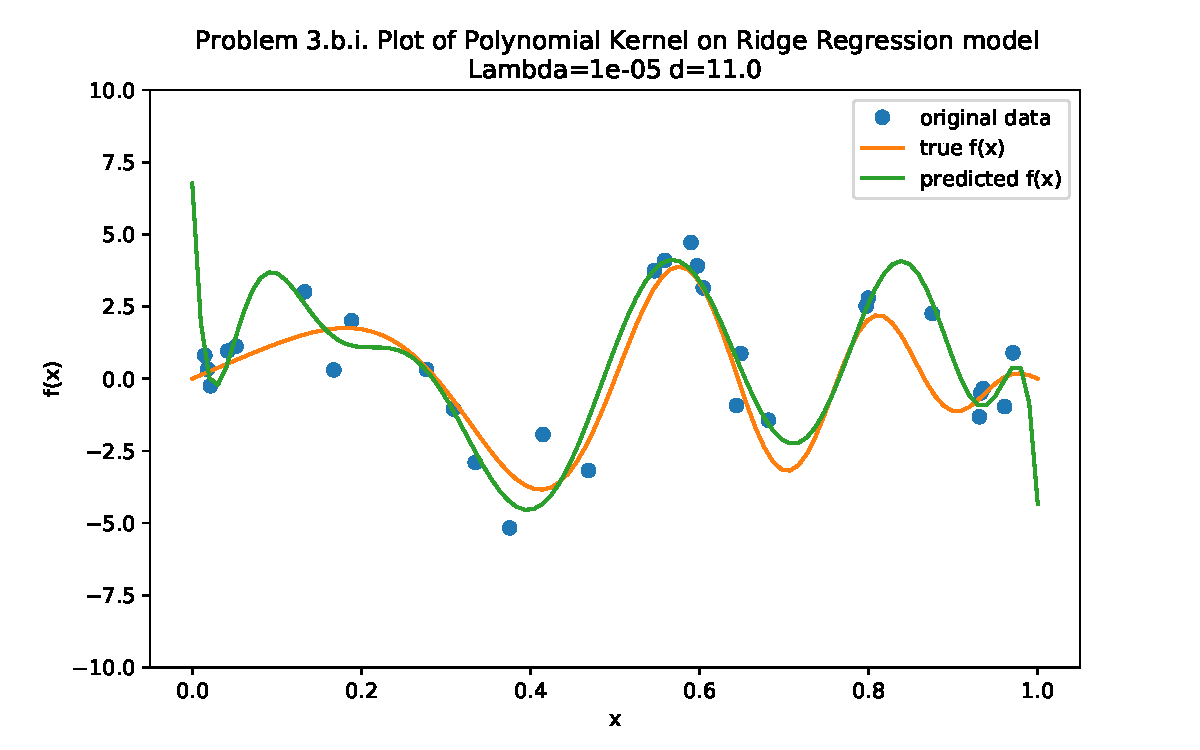
\includegraphics[width=0.8\linewidth]{../plots/3bi.pdf}
	    \caption{}
	\end{figure}
	\begin{figure}[h!]
	    \centering
	    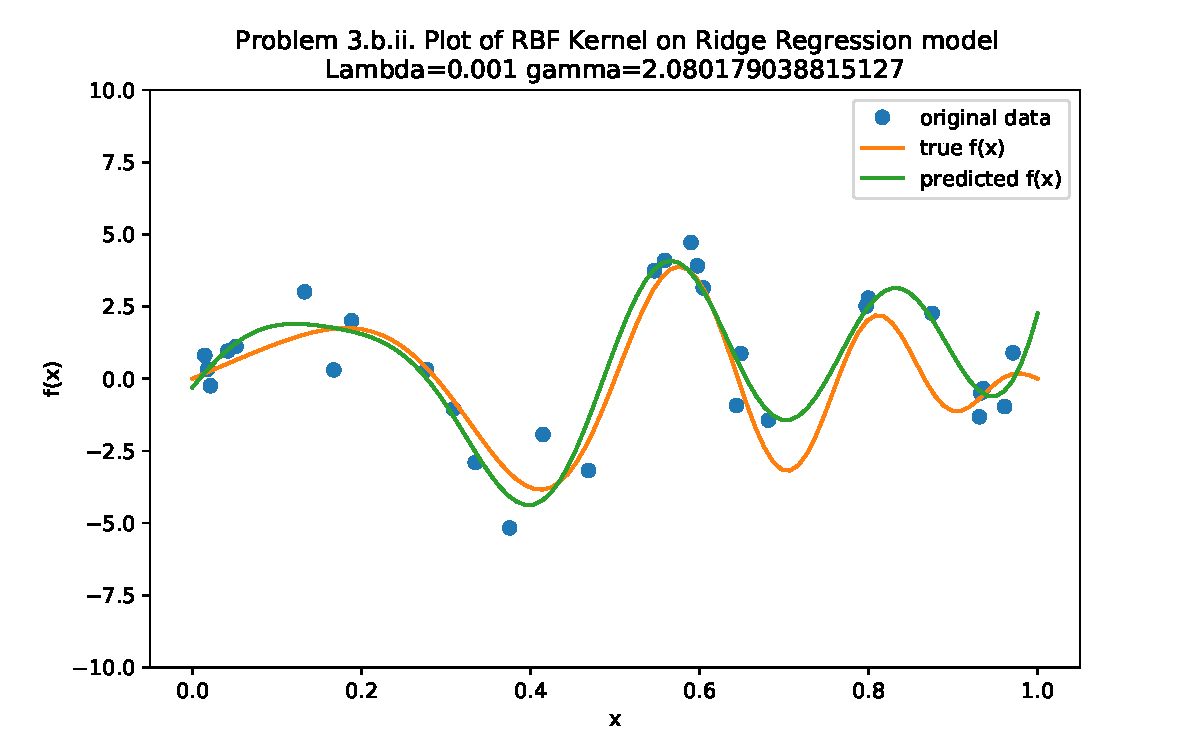
\includegraphics[width=0.8\linewidth]{../plots/3bii.pdf}
	    \caption{}
	\end{figure} \\
\end{enumerate}

{\bf Problem 3: Code}
\lstinputlisting[language=Python]{../code/p3.py}



\noindent\rule{\textwidth}{1pt}\vspace{0.75mm}
{\bf Problem 4}
{\bf Problem 4: Answers}

\begin{enumerate}
    \item
	    $\lambda_1$: 5.148333441485338 \\
	    $\lambda_2$: 3.7299894906022617 \\
	    $\lambda_{10}$: 1.250010757212031 \\
	    $\lambda_{30}$: 0.36492647617793883 \\
	    $\lambda_{50}$: 0.16962131566853172 \\
	    $\sum_{i=1}^d \lambda_i$: 52.83384400094484
    \item Show a general formula for the rank-$k$ PCA approximation of $x$.
	\begin{align*}
	    \Sigma &= \frac{1}{n} \left( X_{\textrm{train}} - \mathbf{1} \mu^T \right)^T \left( X_{\textrm{train}} - \mathbf{1} \mu^T \right) \\
		&= \frac{1}{n} \left( U S V^T \right)^T \left( U S V^T \right) \tag*{Substitute SVD of $X_{\textrm{train}} - \mathbf{1} \mu^T$} \\
		&= \frac{1}{n} V S U^T U S^T V^T \\
		&= \frac{1}{n} V S^2 V^T \\
		&= \frac{1}{n} \left( X_{\textrm{train}} - \mathbf{1} \mu^T \right) \left( X_{\textrm{train}} - \mathbf{1} \mu^T \right) V \\
		&= \frac{1}{n} V S^2 \\
		&= \frac{1}{n} V D
	\end{align*}
	Now consider that since $S$ is a diagonal matrix,
	    \begin{equation*}
		S^2 = 
		    \begin{bmatrix}
			s_1^2 & 0 & 0 & ... \\
			0 & s_2^2 & ... & 0 \\
			0 & 0 & ... & ... \\
			0 & 0 & ... & 0
		    \end{bmatrix}	
	    \end{equation*}
	Which implies that 
	    \begin{equation*}
		\frac{1}{n} D = 
		    \begin{bmatrix}
			\frac{1}{n} d_1 & 0 & 0 & ... \\
			0 & \frac{1}{n} d_2 & ... & 0 \\
			0 & 0 & ... & ... \\
			0 & 0 & ... & 0
		    \end{bmatrix}	
	    \end{equation*}
	Therefore, let $\lambda_i = \frac{1}{n} d_i$ where $\lambda_i$ is the $i$-th eigenvalue of $V$
	    \begin{align*}
		\Sigma V &= \frac{1}{n} V D \\
			&= V
			\begin{bmatrix}
			    \lambda_1 & 0 & 0 & ... \\
			    0 & \lambda_2 & ... & 0 \\
			    0 & 0 & ... & ... \\
			    0 & 0 & ... & 0
			\end{bmatrix} \\
		\Sigma v_i &= \lambda_i v_i
	    \end{align*}
	So $\left( X_{\textrm{train}} - \mathbf{1} \mu^T \right)$ where $x_i \in \R$ can be projected onto $k$ dimensions by using the first $k$ eigenvectors of $V$ to compute the minimum reconstruction error. 
	Thus, a general formula for the rank-$k$ PCA approximation for $x$ can be written $$ \bar{x} = V_k V_k^T \left(x_i - \mu^T \right) + \mu $$
    \item See Figures 4 and 5
	\begin{figure}[h!]
	    \centering
	    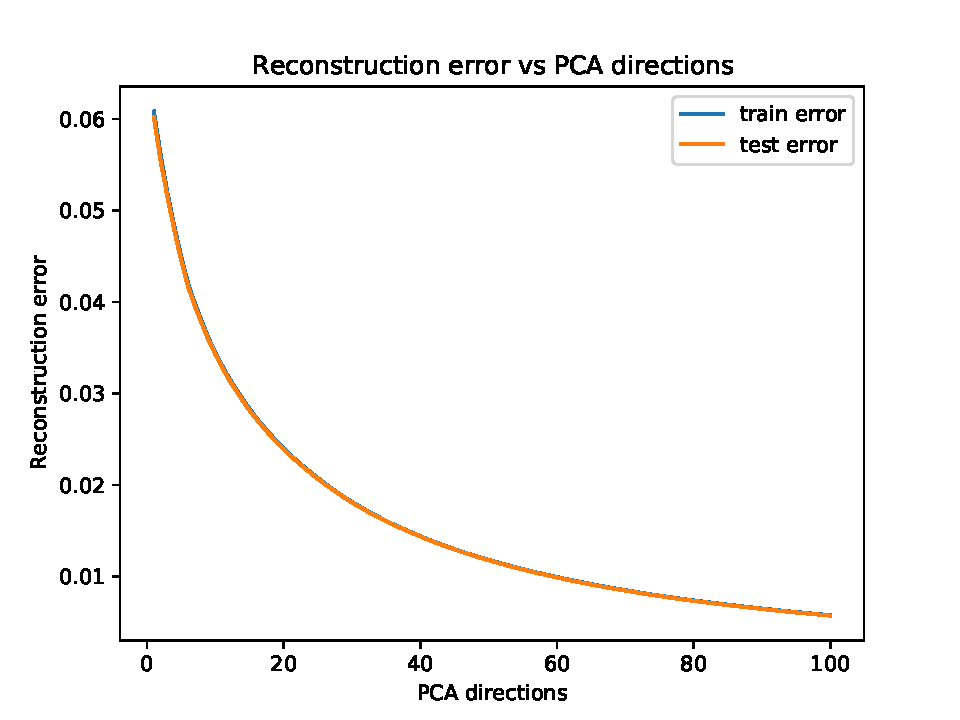
\includegraphics[width=0.8\linewidth]{../figures/a4_re.pdf}
	    \caption{}
	\end{figure}
	\begin{figure}[h!]
	    \centering
	    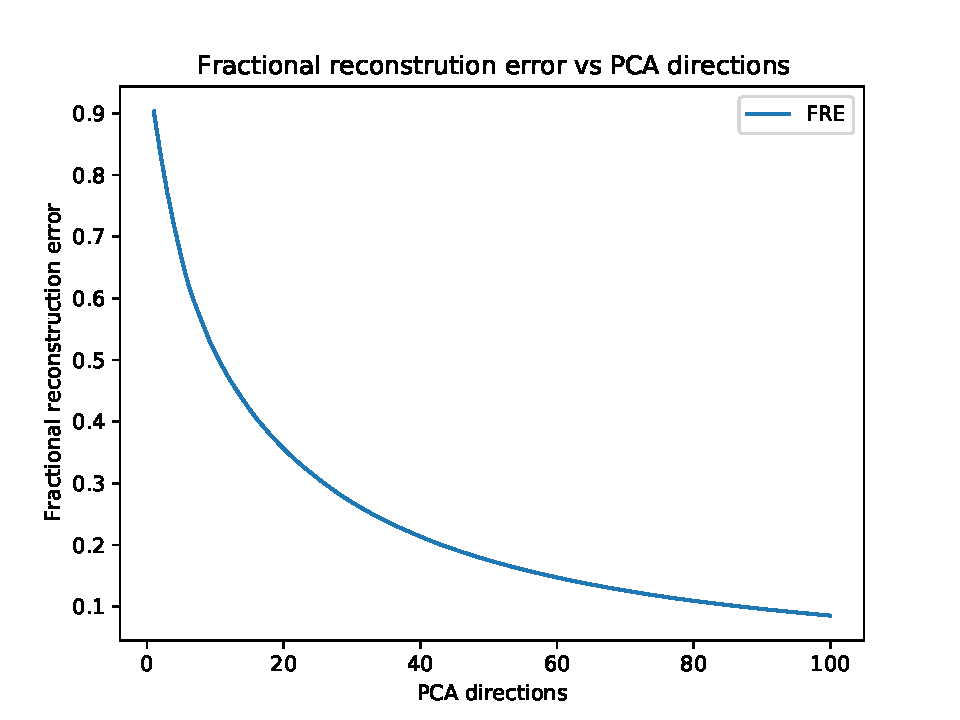
\includegraphics[width=0.8\linewidth]{../figures/a4_fre.pdf}
	    \caption{}
	\end{figure}
    \item See Figure 6. These represent the first 10 eigenvectors in the single value decomposition of the sample covariance of training examples. They correspond to the most significant entries in the training dataset and so contain overlapping, repeated, and missing digits.
	\begin{figure}[h!]
	    \centering
	    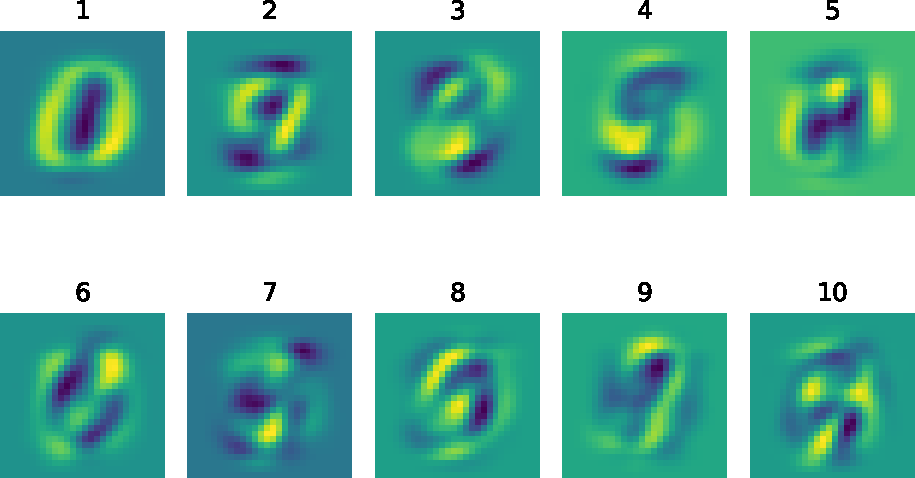
\includegraphics[width=0.8\linewidth]{../figures/a4_eigenvectors.pdf}
	    \caption{}
	\end{figure}
    \item See Figure 7. Increasing k improves the fidelity of the reconstruction. 
    \begin{figure}[h!]
	    \centering
	    \caption{}
	    
\includegraphics[width=0.6\linewidth]{../figures/a4_actual.pdf}
	    \caption*{Actual}
	    
\includegraphics[width=0.6\linewidth]{../figures/a4_recon_5.pdf}
	    \caption*{k=5}
	    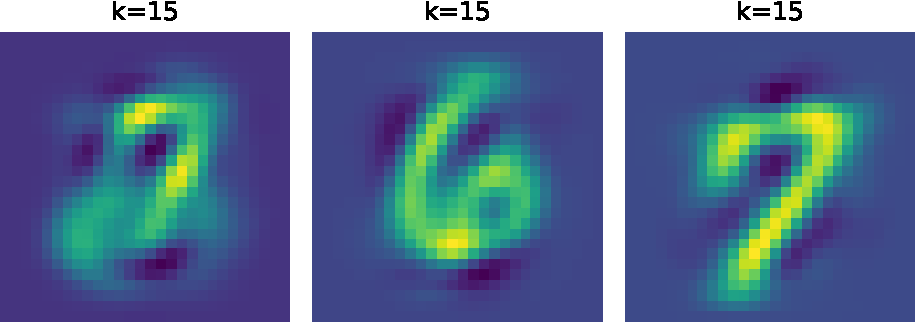
\includegraphics[width=0.6\linewidth]{../figures/a4_recon_15.pdf}
	    \caption*{k=15}
	    
\includegraphics[width=0.6\linewidth]{../figures/a4_recon_40.pdf}
	    \caption*{k=40}
	    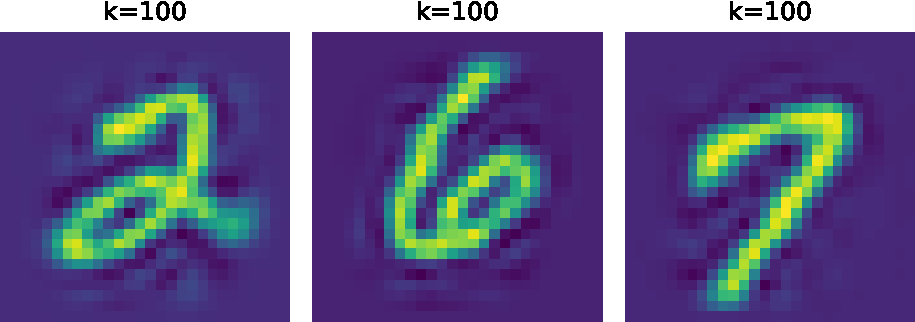
\includegraphics[width=0.6\linewidth]{../figures/a4_recon_100.pdf}
	    \caption*{k=100}
	\end{figure}
\end{enumerate}

{\bf Problem 4: Code}
\begin{quote}
    \lstinputlisting[language=Python]{../code/a4.py}
\end{quote}



\section*{Lasso on a real dataset}
\noindent\rule{\textwidth}{1pt}\vspace{0.75mm}
5. Suppose we have $N$ labeled samples $S = \{(x_i,y_i)\}_{i=1}^N$
drawn i.i.d. from an underlying distribution $\mathcal{D}$. Suppose we
decide to break this set into a set $S_{\textrm{train}}$ of size
$N_{\textrm{train}}$ and a set $S_{\textrm{test}}$ of size
$N_{\textrm{test}}$ samples for our training and test set, so
$N = N_{\textrm{train}} + N_{\textrm{test}}$, and $S = S_{\textrm{train}} \cup S_{\textrm{test}}$.  Recall the definition
of the true least squares error of $f$:
\[
  \epsilon(f) = 
  \mathbb{E}_{(x,y) \sim \mathcal{D}} [ (f(x) -y)^2 ],
\]
where the subscript $(x,y) \sim \mathcal{D}$ makes clear that our
input-output pairs are sampled according to $\mathcal{D}$.
Our training and test losses are defined as:
\begin{align*}
\widehat{\epsilon}_{\textrm{train}}(f) &=
\frac{1}{N _{\textrm{train}}} \sum_{(x,y)\in S_{\textrm{train}}}     (f(x) -y)^2
\\
  \widehat{\epsilon}_{\textrm{test}}(f) &=
  \frac{1}{N _{\textrm{test}}} \sum_{(x,y)\in S_{\textrm{test}}}     (f(x) -y)^2  
\end{align*}
We then train our algorithm (for example, using linear least squares
regression) using the training set to obtain $\widehat{f}$.


\begin{enumerate}
\item \points{6} (bias: the test error) Define $\E_{\textrm{train}}$ as the expectation over all training set $S_{\textrm{train}}$ and $\E_{\textrm{test}}$ as the expectation over all testing set $S_{\textrm{test}}$. For all fixed $f$ (before we've seen any data) show that
\[\E_{\textrm{train}}[ \widehat{\epsilon}_{\textrm{train}}(f) ] = \E_{\textrm{test}}[ \widehat{\epsilon}_{\textrm{test}}(f) ] = \epsilon(f).\] 
Use a similar line of reasoning to show that the test error is an
unbiased estimate of our true error for $\hat{f}$. Specifically, show
that:
\[
  \mathbb{E}_{\textrm{test}}[\widehat{\epsilon}_{\textrm{test}}(\widehat{f})] = \epsilon(\widehat{f})
\]
\begin{itemize}
    \item Show that $\E_{\textrm{train}}[ \widehat{\epsilon}_{\textrm{train}}(f) ] = \epsilon(f)$.
    \item[] 
	\begin{align*}
	    \E_{\textrm{train}}[ \widehat{\epsilon}_{\textrm{train}}(f) ] 
		&=  \E_{\textrm{train}} \left[ \frac{1}{N_{\textrm{train}}} \sum_{(x, \, y)\in S_{\textrm{train}}} \left( f(x) - y \right)^2 \right] \tag*{Given} \\
		&= \frac{1}{N_{\textrm{train}}} \, \E_{\textrm{train}} \left[  \sum_{(x, \, y)\in S_{\textrm{train}}} \left( f(x) - y \right)^2 \right] \tag*{By Linearity of Expectation} \\
		&= \frac{1}{N_{\textrm{train}}} \, N_{\textrm{train}} \, \E_{(x,\, y) \sim \mathcal{D}} \left[  \left( f(x) - y \right)^2 \right] \tag*{Since the points in $S_{\textrm{train}}$ are iid} \\
		&= \E_{(x,y) \sim \mathcal{D}} \left[ (f(x) -y)^2 \right] \\
		&= \epsilon(f)
	\end{align*}
    \item Show that $\E_{\textrm{test}}[ \widehat{\epsilon}_{\textrm{test}}(f) ] = \epsilon(f)$.
    \item[] 
	\begin{align*}
	    \E_{\textrm{test}}[ \widehat{\epsilon}_{\textrm{test}}(f) ] 
		&=  \E_{\textrm{test}} \left[ \frac{1}{N_{\textrm{test}}} \sum_{(x, \, y)\in S_{\textrm{test}}} \left( f(x) - y \right)^2 \right] \tag*{Given} \\
		&= \frac{1}{N_{\textrm{test}}} \, \E_{\textrm{test}} \left[  \sum_{(x, \, y)\in S_{\textrm{test}}} \left( f(x) - y \right)^2 \right] \tag*{By Linearity of Expectation} \\
		&= \frac{1}{N_{\textrm{test}}} \, N_{\textrm{test}} \, \E_{(x,\, y) \sim \mathcal{D}} \left[  \left( f(x) - y \right)^2 \right] \tag*{Since the points in $S_{\textrm{test}}$ are iid} \\
		&= \E_{(x,y) \sim \mathcal{D}} \left[ (f(x) -y)^2 \right] \\
		&= \epsilon(f)
	\end{align*}
    \item Since $\E_{\textrm{train}}[ \widehat{\epsilon}_{\textrm{train}}(f) ] = \epsilon(f)$ and $\E_{\textrm{test}}[ \widehat{\epsilon}_{\textrm{test}}(f) ] = \epsilon(f)$, thus $$\boxed{ \E_{\textrm{train}}[ \widehat{\epsilon}_{\textrm{train}}(f) ] = \E_{\textrm{test}}[ \widehat{\epsilon}_{\textrm{test}}(f) ] = \epsilon(f) } $$
    \item Show that $\E_{\textrm{test}}[ \widehat{\epsilon}_{\textrm{test}}(\widehat{f}) ] = \epsilon(\widehat{f})$.
    \item[] 
	\begin{align*}
	    \E_{\textrm{test}}[ \widehat{\epsilon}_{\textrm{test}}(\widehat{f}) ] 
		&=  \E_{\textrm{test}} \left[ \frac{1}{N_{\textrm{test}}} \sum_{(x, \, y)\in S_{\textrm{test}}} \left( \widehat{f}(x) - y \right)^2 \right] \tag*{Given} \\
		&= \frac{1}{N_{\textrm{test}}} \, \E_{\textrm{test}} \left[  \sum_{(x, \, y)\in S_{\textrm{test}}} \left( \widehat{f}(x) - y \right)^2 \right] \tag*{By Linearity of Expectation} \\
		&= \frac{1}{N_{\textrm{test}}} \, N_{\textrm{test}} \, \E_{(x,\, y) \sim \mathcal{D}} \left[  \left( \widehat{f}(x) - y \right)^2 \right] \tag*{Since the points in $S_{\textrm{test}}$ are iid} \\
		&= \E_{(x,y) \sim \mathcal{D}} \left[ (\widehat{f}(x) -y)^2 \right] \\
		&= \epsilon(\widehat{f})
	\end{align*}
    \item[] Thus, $$\boxed{ \E_{\textrm{test}}[ \widehat{\epsilon}_{\textrm{test}}(\widehat{f}) ] = \epsilon(\widehat{f}) } $$
\end{itemize}



\item \points{5} (bias: the train/dev error) Is the above equation true (in general) with regards to the
  training loss? Specifically, does $\mathbb{E}_{\textrm{train}}[\widehat{\epsilon}_{\textrm{train}}(\widehat{f})]$ equal $\mathbb{E}_{\textrm{train}}[ \epsilon(\widehat{f})]$? If so, why? If not, give a clear argument as
  to where your previous argument breaks down.
\begin{quote}
    In general {\bf it is not true} that $\E_{\text{train}}[ \widehat{\epsilon}_{\text{train}} ( \widehat{f} )] = \E_{\text{train}} [ \epsilon (\widehat{f}) ]$. This is because, above, to go from $\frac{1}{N_{\textrm{test}}} \, \E_{\textrm{test}} \left[  \sum_{(x, \, y)\in S_{\textrm{test}}} \left( \widehat{f}(x) - y \right)^2 \right]$ to $\frac{1}{N_{\textrm{test}}} \, N_{\textrm{test}} \, \E_{(x,\, y) \sim \mathcal{D}} \left[  \left( \widehat{f}(x) - y \right)^2 \right]$ we had to know that $x_i$, $y_i$, and $\widehat{f}$ were iid from $S_{\textrm{train}}$. We knew this to be the case above because we're told that $x_i$ and $y_i$ are iid and that $\widehat{f}$ was found using only training data. However, since we don't always know how $\widehat{f}$ was found, we can't always assume that $\widehat{f}$ is iid from $S_{\textrm{train}}$, and thus it's not generally true that $\E_{\text{train}}[ \widehat{\epsilon}_{\text{train}} ( \widehat{f} )] = \E_{\text{train}} [ \epsilon (\widehat{f}) ]$.
\end{quote}



\item \points{8} Let $\mathcal{F} = (f_1, f_2,\dots)$ be a collection of functions and let $\widehat{f}_{\textrm{train}}$ minimize the training error such that $\widehat{\epsilon}_{\textrm{train}}(\widehat{f}_{\textrm{train}}) \leq \widehat{\epsilon}_{\textrm{train}}(f)$ for all $f \in \mathcal{F}$.
Show that
\begin{align*}
\E_{\text{train}}[ \widehat{\epsilon}_{\textrm{train}}(\widehat{f}_{\textrm{train}}) ] \leq \E_{\text{train,test}}[ \widehat{\epsilon}_{\textrm{test}}(\widehat{f}_{\textrm{train}}) ].
\end{align*}
(Hint: 
note that
\begin{align*}
\E_{\text{train,test}}[ \widehat{\epsilon}_{\textrm{test}}(\widehat{f}_{\textrm{train}}) ] &= \sum_{f \in \mathcal{F}} \E_{\text{train,test}}[ \widehat{\epsilon}_{\textrm{test}}(f) \1\{ \widehat{f}_{\textrm{train}} = f\}] \\
&= \sum_{f \in \mathcal{F}} \E_{\text{test}}[ \widehat{\epsilon}_{\textrm{test}}(f) ] \E_{\text{train}}[ \1\{\widehat{f}_{\textrm{train}} = f \}]\\ &= \sum_{f \in \mathcal{F}} \E_{\text{test}}[ \widehat{\epsilon}_{\textrm{test}}(f) ] \P_{\text{train}}(\widehat{f}_{\textrm{train}} = f )
\end{align*}
where the second equality follows from the independence between the train and test set.)\\
\begin{quote}
    {\bf Lemma}: $\widehat{\epsilon}_{\textrm{train}} ( \widehat{f}_{\textrm{train}} ) \leq \widehat{\epsilon}_{\textrm{train}} (f) \, \forall f \in \mathcal{F} \implies \E \left[ \widehat{\epsilon}_{\textrm{train}} ( \widehat{f}_{\textrm{train}} ) \right] \leq \E \left[ \widehat{\epsilon}_{\textrm{train}} (f) \right] \, \forall f \in \mathcal{F}$
\end{quote}

\begin{align*}
    \E_{\textrm{train}} \left[ \widehat{\epsilon}_{\textrm{train}} ( \widehat{f}_{\textrm{train}} ) \right]
	&= \E_{\textrm{train}} \left[ \widehat{\epsilon}_{\textrm{train}} ( \widehat{f}_{\textrm{train}} ) \right] * 1 \tag*{Trivially} \\
	&= \E_{\textrm{train}} \left[ \widehat{\epsilon}_{\textrm{train}} ( \widehat{f}_{\textrm{train}} ) \right] \sum_{f \in \mathcal{F}} \P \left( \widehat{f}_{\textrm{train}} = f \right) \tag*{Sum of PMF = 1} \\
	&= \sum_{f \in \mathcal{F}} \E_{\textrm{train}} \left[ \widehat{\epsilon}_{\textrm{train}} ( \widehat{f}_{\textrm{train}} ) \right] \P \left( \widehat{f}_{\textrm{train}} = f \right) \tag*{By Linearity of Expectation} \\
	&\leq \sum_{f \in \mathcal{F}} \E_{\textrm{train}} \left[ \widehat{\epsilon}_{\textrm{train}} ( f ) \right] \P \left( \widehat{f}_{\textrm{train}} = f \right) \tag*{From above lemma} \\
	&= \sum_{f \in \mathcal{F}} \E_{\textrm{test}} \left[ \widehat{\epsilon}_{\textrm{test}} ( f ) \right] \P \left( \widehat{f}_{\textrm{train}} = f \right) \tag*{Proven in a.} \\
	&= \sum_{f \in \mathcal{F}} \E_{\textrm{test}} \left[ \widehat{\epsilon}_{\textrm{test}} ( f ) \right] \E_{\textrm{train}} \left[ \1 \{ \widehat{f}_{\textrm{train}} = f \} \right] \tag*{Given in hint} \\
	&= \sum_{f \in \mathcal{F}} \E_{\textrm{train,test}} \left[ \widehat{\epsilon}_{\textrm{test}} ( f ) \,\1 \{ \widehat{f}_{\textrm{train}} = f \} \right] \tag*{Given in hint} \\
	&= \E_{\textrm{train,test}} \left[ \widehat{\epsilon}_{\textrm{test}} ( \widehat{f}_{\textrm{train}} ) \right] \tag*{Given in hint}
\end{align*}

\begin{quote}
    Thus,$$\boxed{ \E_{\textrm{train}} \left[ \widehat{\epsilon}_{\textrm{train}} ( \widehat{f}_{\textrm{train}} ) \right] \leq \E_{\textrm{train,test}} \left[ \widehat{\epsilon}_{\textrm{test}} ( \widehat{f}_{\textrm{train}} ) \right] }$$
\end{quote}




\end{enumerate}  

\lstinputlisting[language=Python]{body/p5.py}

\noindent\rule{\textwidth}{1pt}\vspace{0.75mm}
{\bf Problem 6}
\begin{quote}
    \FloatBarrier
    \begin{figure}
	\captionsetup{labelformat=empty}
	\caption{Results of training Polynomial Regression model of degree d = 8.}
   	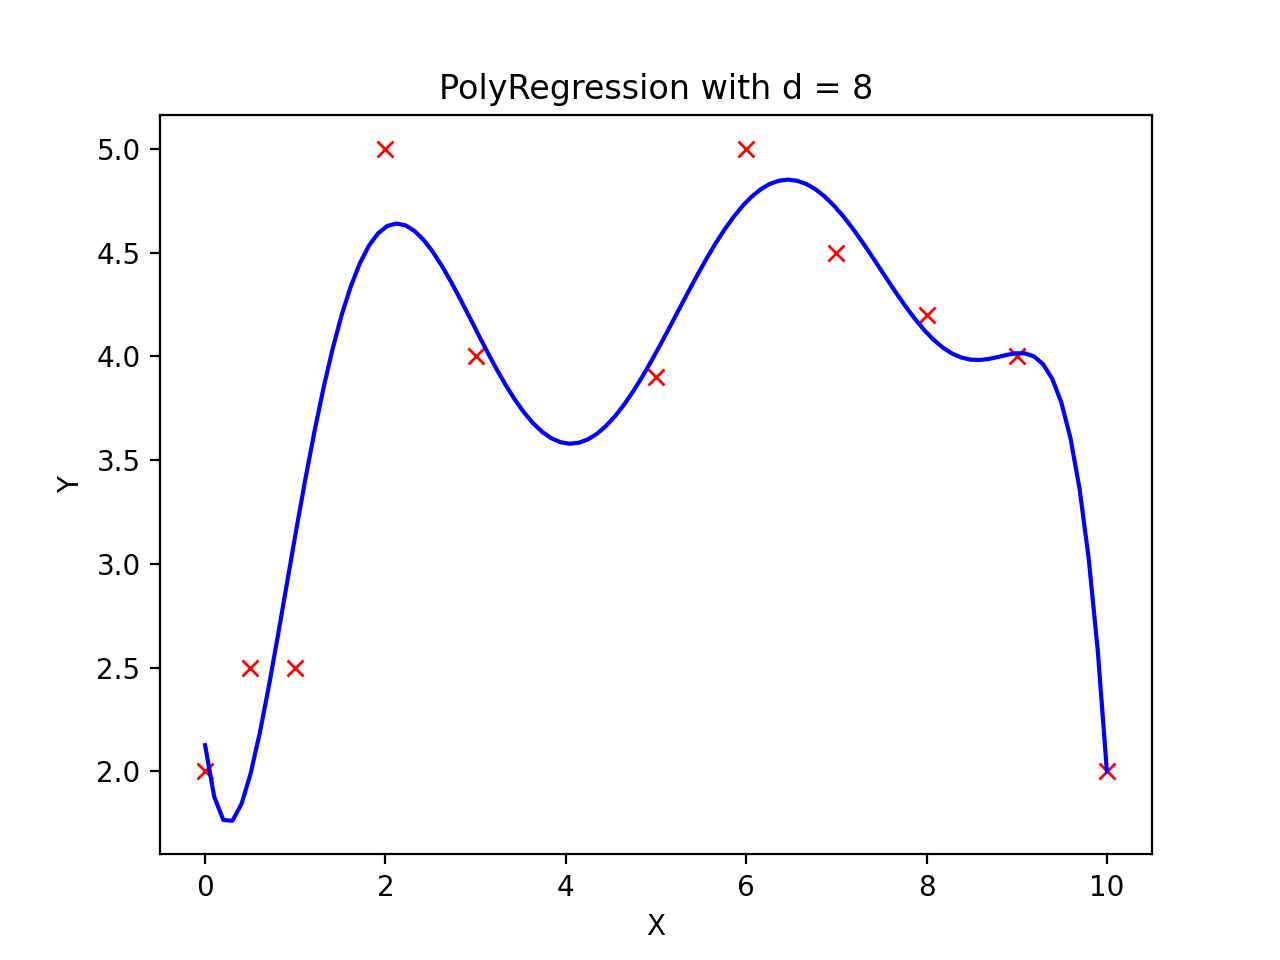
\includegraphics[scale=0.5]{./images/fig1.png} 
	\centering
    \end{figure}
    \FloatBarrier
\end{quote}


\lstinputlisting[language=Python]{body/p6.py}

\section*{Logistic Regression}
\noindent\rule{\textwidth}{1pt}\vspace{0.75mm}
7. \points{15} In this problem we will examine the bias-variance tradeoff through learning curves. Learning curves provide a valuable mechanism for evaluating the bias-variance tradeoff. Implement the \texttt{learningCurve()} function in \texttt{polyreg.py} to compute the learning curves for a given training/test set.  The \texttt{learningCurve(Xtrain, ytrain, Xtest, ytest, degree, regLambda)} function should take in the training data (\texttt{Xtrain}, \texttt{ytrain}), the testing data (\texttt{Xtest}, \texttt{ytest}), and values for the polynomial degree $d$ and regularization parameter $\lambda$. 

The function should return two arrays, \texttt{errorTrain} (the array of training errors) and \texttt{errorTest} (the array of testing errors).  The $i^{th}$ index (start from 0) of each array should return the training error (or testing error) for learning with $i +1$ training instances.  Note that the 0$^{th}$ index actually won't matter, since we typically start displaying the learning curves with two or more instances.


\vspace{.1in}
When computing the learning curves, you should learn on \texttt{Xtrain}[0:$i$] for $i = 1, \ldots, \text{numInstances}(\texttt{Xtrain})+1$, each time computing the testing error over the {\bf entire} test set.  There is no need to shuffle the training data, or to average the error over multiple trials -- just produce the learning curves for the given training/testing sets with the instances in their given order.  Recall that the error for regression problems is given by
\begin{equation}
\frac{1}{n} \sum_{i=1}^n (h_{\bm{\theta}}(\mathbf{x}_i) - y_i)^2 \enspace .
\end{equation}

Once the function is written to compute the learning curves, run the \texttt{test\_polyreg\_learningCurve.py} script to plot the learning curves for various values of $\lambda$ and $d$.  You should see plots similar to the following:
\begin{figure}[ht!]
      \centering
      \vspace{-1em}
      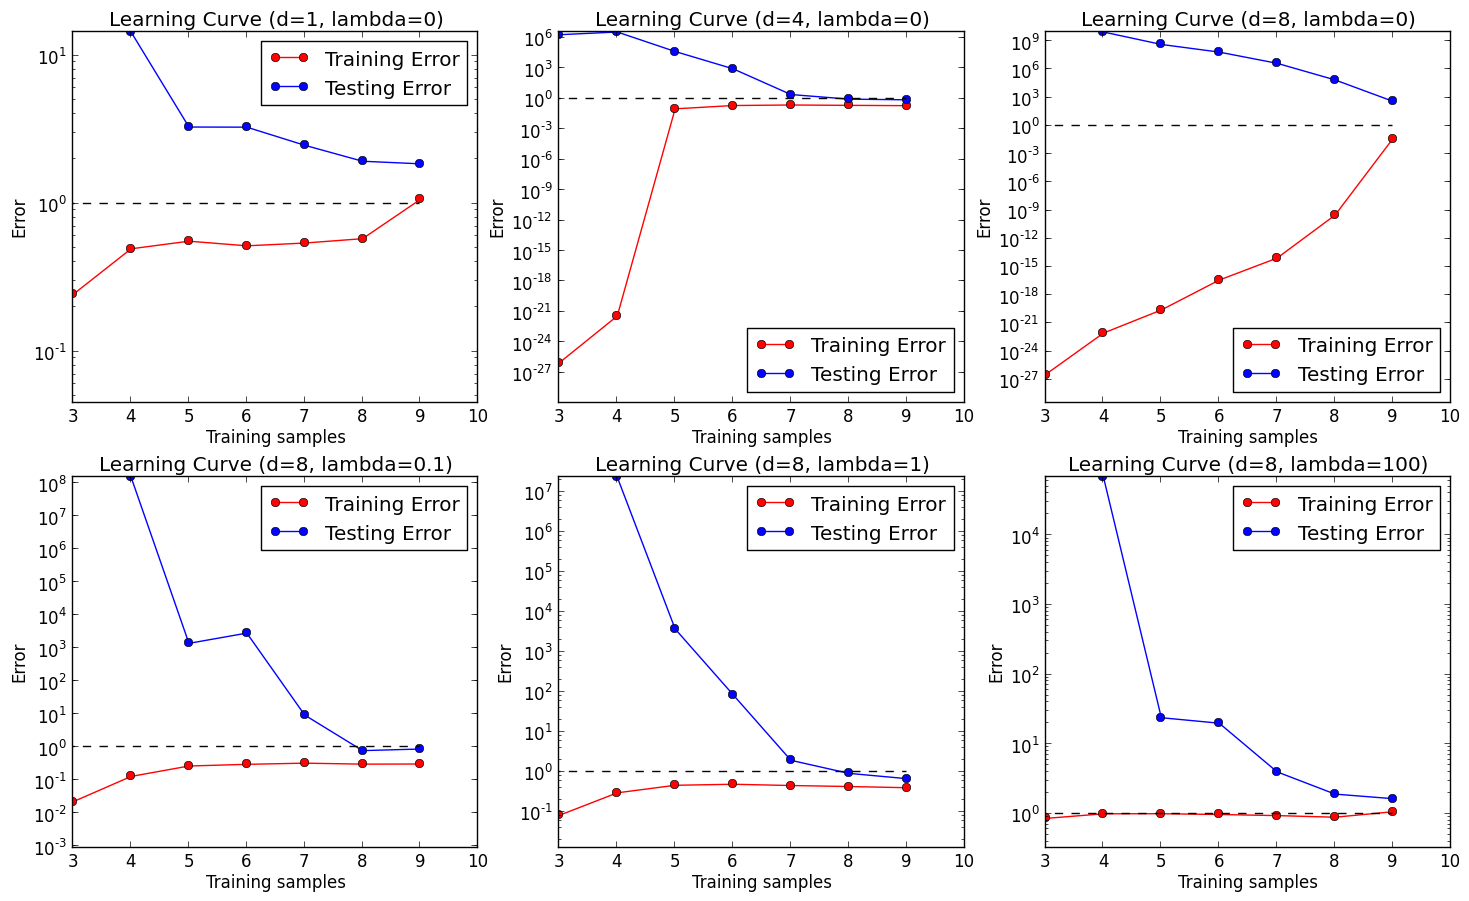
\includegraphics[width=\textwidth]{images/polyregLearningCurves.png}
      \vspace{-1em}
    \end{figure}

Notice the following:
\begin{itemize}
\item The y-axis is using a log-scale and the ranges of the y-scale are all different for the plots.  The dashed black line indicates the $y=1$ line as a point of reference between the plots.
\item The plot of the unregularized model with $d = 1$ shows poor training error, indicating a high bias (i.e., it is a standard univariate linear regression fit).
\item The plot of the unregularized model ($\lambda = 0$) with $d = 8$ shows that the training error is low, but that the testing error is high.  There is a huge gap between the training and testing errors caused by the model overfitting the training data, indicating a high variance problem.
\item As the regularization parameter increases (e.g., $\lambda = 1$) with $d = 8$, we see that the gap between the training and testing error narrows, with both the training and testing errors converging to a low value.  We can see that the model fits the data well and generalizes well, and therefore does not have either a high bias or a high variance problem.  Effectively, it has a good tradeoff between bias and variance.
\item Once the regularization parameter is too high ($\lambda = 100$), we see that the training and testing errors are once again high, indicating a poor fit.  Effectively, there is too much regularization, resulting in high bias.
\end{itemize}

\textbf{Please include both your code and the generated plots in your homework.} Make absolutely certain that you understand these observations, and how they relate to the learning curve plots.  In practice, we can choose the value for $\lambda$ via cross-validation to achieve the best bias-variance tradeoff.

\begin{quote}
    \FloatBarrier
    \begin{figure}
	\captionsetup{labelformat=empty}	
	\caption{Results of training and testing error over multiple degrees d and lambdas $\lambda$.}
	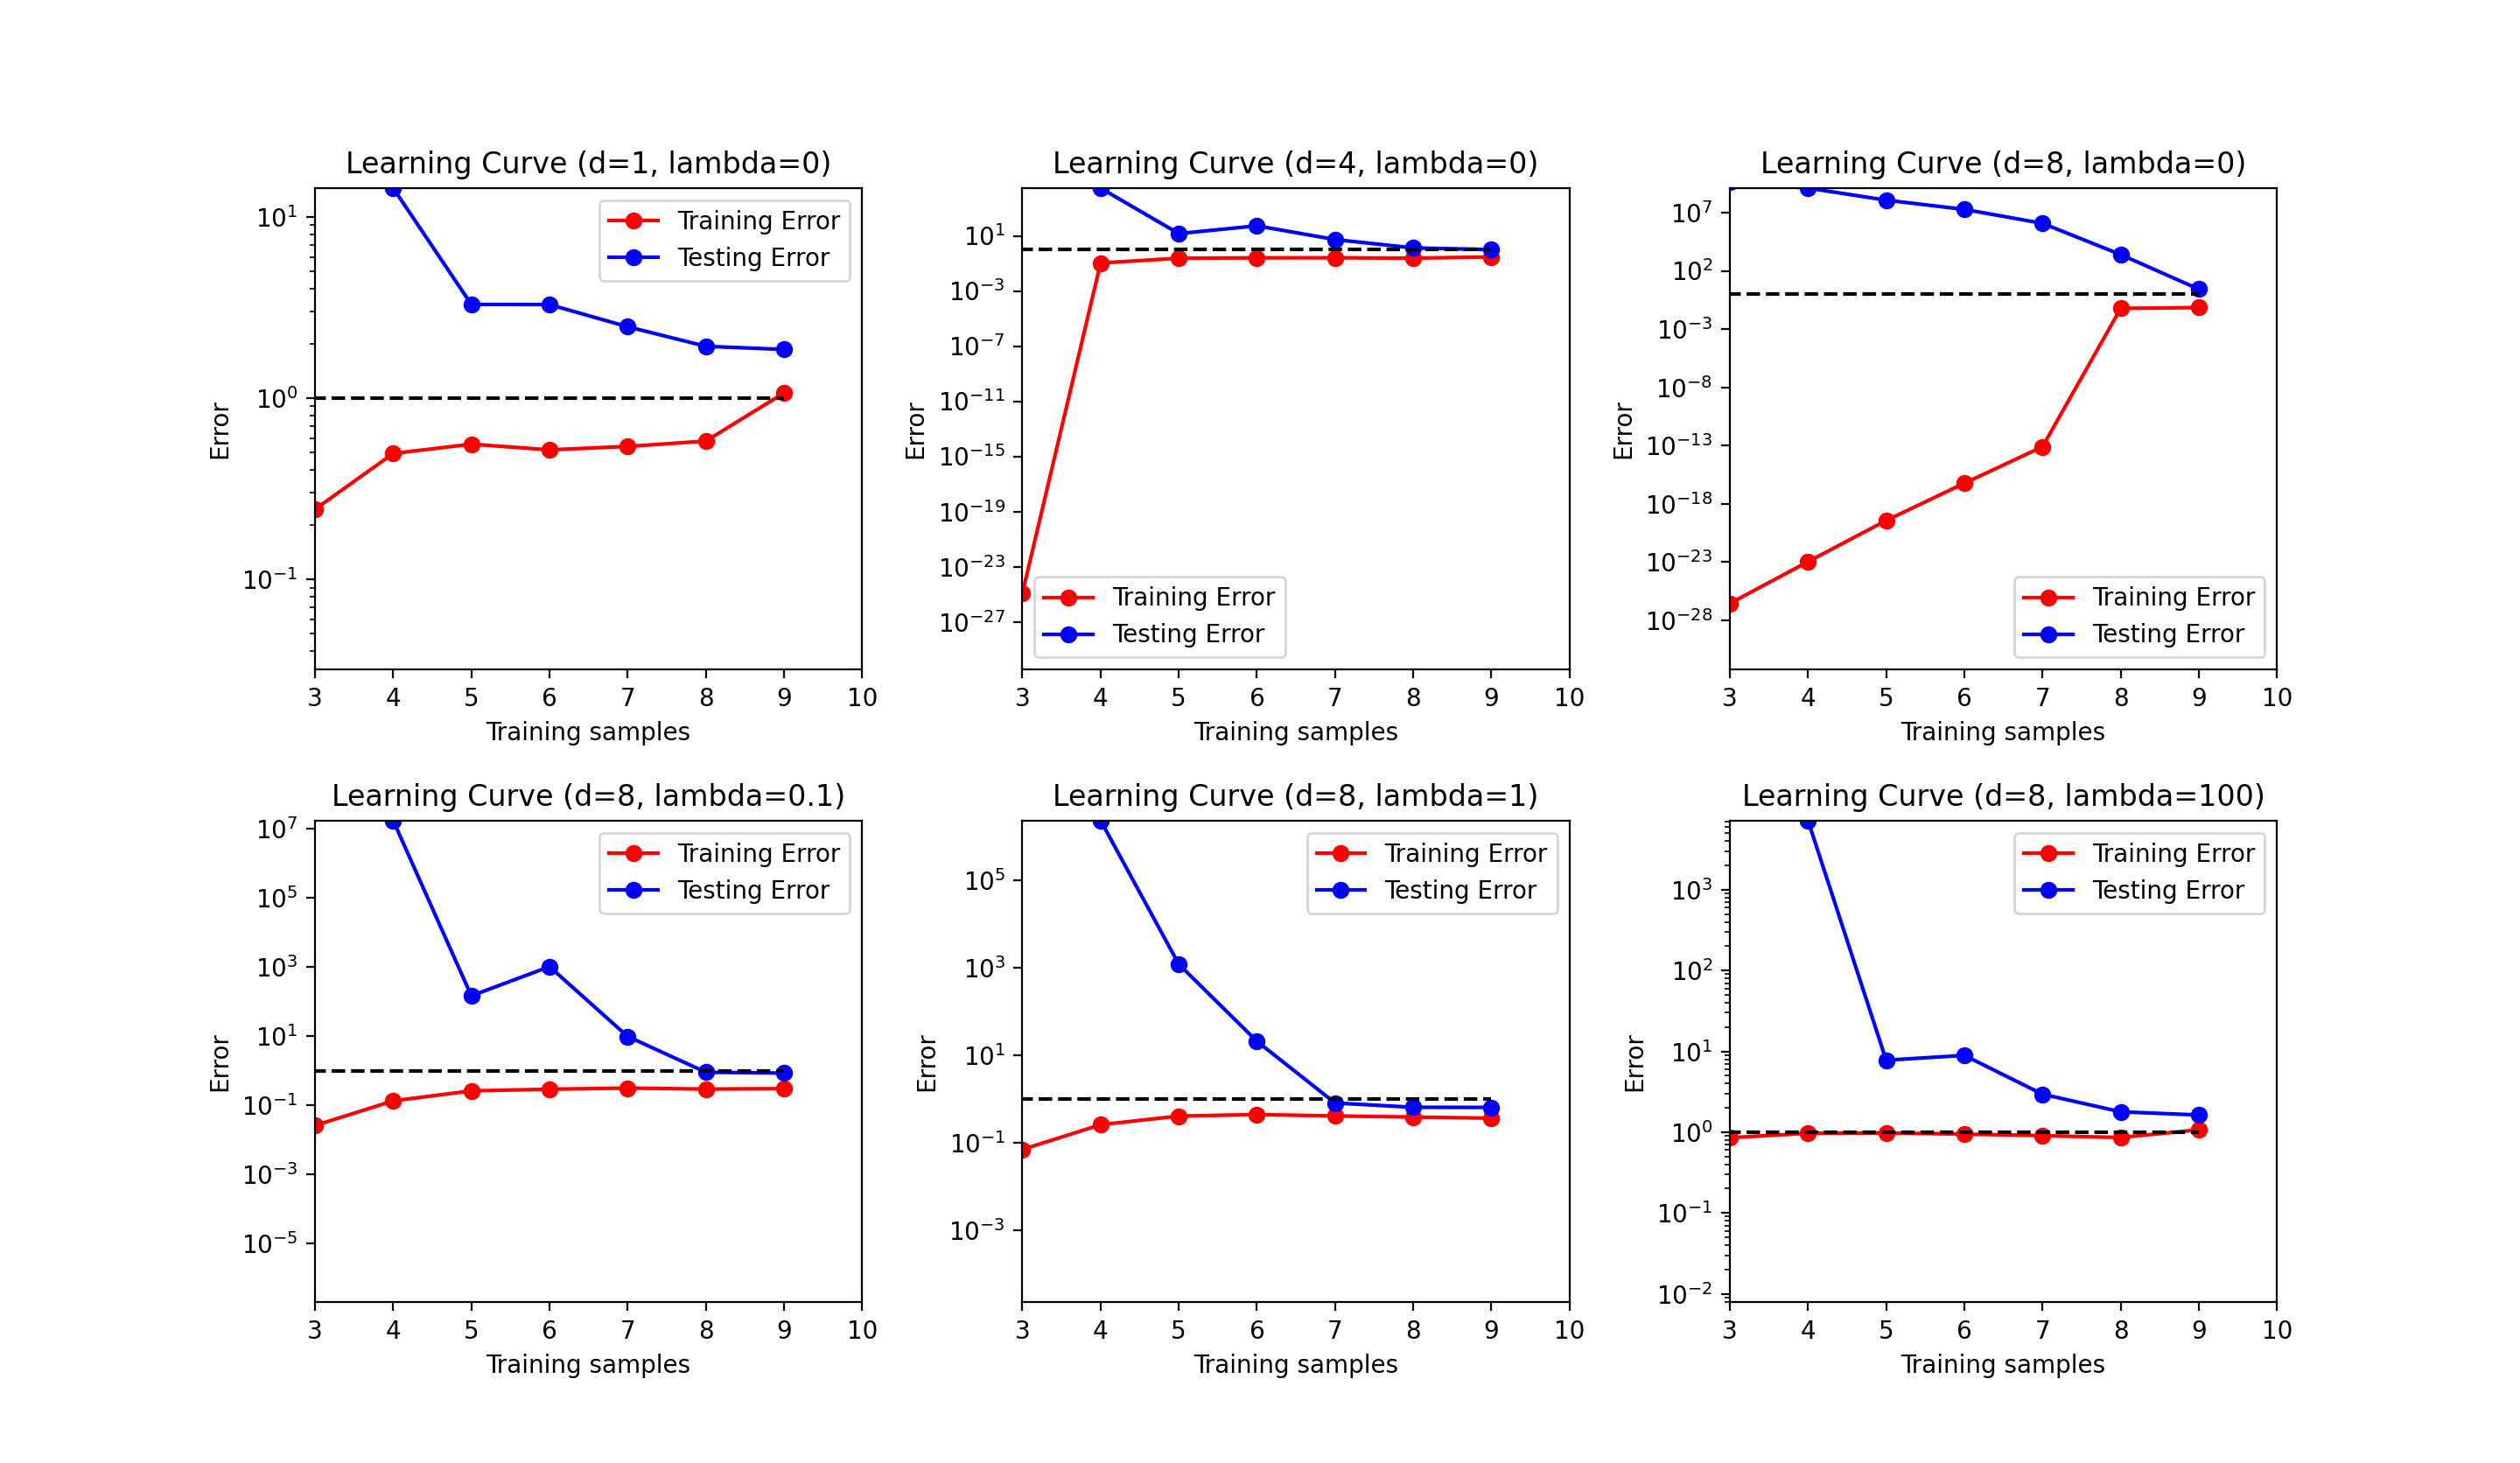
\includegraphics[scale=0.5]{./images/fig2.png} 
	\centering
    \end{figure}
    \FloatBarrier
    \begin{itemize}
	\item[] \lstinputlisting[language=Python]{body/polyreg.py}
    \end{itemize}
\end{quote}



\lstinputlisting[language=Python]{body/p7.py}

{\bf Additional files used for Problems 5-7}
\lstinputlisting[language=Python]{body/DataManagement.py}
\lstinputlisting[language=Python]{body/GradientDescent.py}
\lstinputlisting[language=Python]{body/Lasso.py}
\lstinputlisting[language=Python]{body/Performance.py}
\lstinputlisting[language=Python]{body/StochasticGradientDescent.py}
\lstinputlisting[language=Python]{body/Supplemental.py}

\end{document}
